\section{Game playing.}
\label{sec:game-playing}

In \sectionref{model} we modeled on-the-job learning as a stochastic game played between the system and the crowd, and defined a reasonable model of the environment and utility for the system to maximize.
We now turn to the problem of actually finding a policy that maximizes the expected utility,
which is, of course, intractable because of the large state space.
In \algorithmref{mcvts}, we propose an approximate Monte Carlo algorithm to find this policy. 

%Having defined the simulation dynamics and utility, we can now define the full game tree,
%which is an extension of our initial example in \figureref{game-tree}~(right).
%The technical challenge here is to incorporate the modeling of continuous time
%into a traditionally discrete game tree.
%A naive approach might be to discretize time and treat each level of the game
%tree as a time step, but this discretization is inefficient.
%Our strategy is to consider only represent game states corresponding to pivotal times $t$
%and model waiting times as random actions played by the crowd.
%%\citep{guo2009continuous}

% Game state, abstract goal
%If it is the crowd's turn,
%then we sample the time of the first ``in flight'' response along with its value.
%Formally, let $F = \{ 1 \le j \le k-1 : q_j \neq \emptyset \wedge r_j = \emptyset \}$ be the ``in flight'' queries.
%Sample $t_j$ according to the time delay model for each $j \in F$
%and take the earliest event $j^* = \arg\min_{j \in F} t_j$;
%the actual response $r_{j^*}$ is drawn independently from the dynamics model conditioned on the queries and responses
%in the state $s$;
%the successor state incorporates $r_{j^*}$ and $t_{j^*}$ and advances time from $\now$ to $t_{j^*}$.

% ARUN: This should be covered when we talk about our game model itself, which introduces the wait action and hence this restriction.
% Technically, the optimal strategy might be to wait for an intermediate amount of time before $t_{j^*}$,
% so our restriction to considering decisions only at response times is an approximation.

%\todo{Improve example}
%The following example shows one path over the states of the game tree corresponding to \figureref{game-tree}~(left),
%where the system takes action $q_2 = 4$ (labeling \nl{str.}) and then the crowd responds
%at time $1.7$ with $r_2 = \scloc$.
%Note that the response $r_1$ for $q_1 = 3$ (\nl{George}) is still pending.
%\begin{center}
%\begin{tabular}{|ll|}
%  \hline $\now = 1$ & \\
%  \hline
%  $q_1 = 3$         & $q_2 = \emptyset$ \\
%  $r_1 = \emptyset$ & $r_2 = \emptyset$ \\
%  \hline
%\end{tabular}
%$\stackrel{\text{\small system}}{\implies}$
%\begin{tabular}{|ll|}
%  \hline $\now = 1$ & \\
%  \hline
%  $q_1 = 3$         & $q_2 = 4$ \\
%  $r_1 = \emptyset$ & $r_2 = \emptyset$ \\
%  \hline
%\end{tabular}
%$\stackrel{\text{\small crowd}}{\implies}$
%\begin{tabular}{|ll|}
%  \hline $\now = 1.7$ & \\
%  \hline
%  $q_1 = 3$         & $q_2 = 4$ \\
%  $r_1 = \emptyset$ & $r_2 = \text{\scloc}$ \\
%  \hline
%\end{tabular}
%\end{center}

%\paragraph{Prediction model.}
% PL: form isn't relevant here since later we use other types of models anyway
%Assume our model
%We consider the family of conditional random fields
%exponential models, a popular class of models that include logistic regression
%and conditional random fields.
%Let $\bx$ be a given input, then the labels $\by = y_1, \ldots, y_n \in \{1,
%\dots, L\}$ are generated by the following conditional distribution:
%\begin{align*}
%  \p(\by \given \bx) 
%  &\propto \exp(\theta^\top \phi(\bx, \by)),
%\end{align*}
%where $\phi(\bx, \by)$ are features
%and $\theta$ are model parameters.
%In this paper, $\p(\by \given \bx) We assume that inference is efficient, which it is
%for our chain-structured models.
%(e.g.\ $\phi$ factorizes over the
%labels $\by$) or otherwise admits efficient marginal computation.

%For example, the model in \figureref{crf} is a linear-chain conditional random
%field. The input is the sequence of words in the tweet and the output is a
%label in the set \scnone, \scres, \scloc{} and \scper. Marginal inference can
%be efficiently computed using the Viterbi algorithm.

%Conventionally, we are given a training dataset $\sD = \{\bx_i, \by_i\}$ and can learn $\theta$ by optimizing the convex log-likelihood objective $\sL(\theta) = \sum_{t=1}^T \log \p(\by\oft{t} \given \bx\oft{t})$.
%In our setting, however, we do not observe the gold labels $\by$. 
%Instead, we can ask the crowd to provide a ``measurement'' for some subset of the labels.
%Let $\Sigma = \{\sigma_i\}$ be the set of possible measurements we can ask the crowd for and 
%let $\by_\sigma \subseteq \by$ be the subset of labels queried.

%\paragraph{Response model.}
%Let $q \in \{1, \ldots, n\}$ be a query on for the label $y_q$.
%We model the response, $r$, with an exponential measurement model:
%\begin{align*}
%  p_\beta(r \given x, y, q) 
%  &\propto \exp \left( \beta^\top\psi(\bx, y_q, r) \right),
%\end{align*}
%where $\beta$ and $\psi$ are extra parameters and features for the human error model. 
%%The choice of an exponential model allows us to simply include measurements as an additional factor.
%\figureref{crf}(c) shows the original graph with additional measurement nodes.
%A simple human error model is to return the true label with probability $1-\epsilon$ and a random label otherwise.
%In our running example, some classes, e.g.\ $\textsc{none}$, are more easily identified than others: in this setting responses can be modeled to be sampled from a confusion matrix.
%
%Finally, we model delay to be drawn from a Gamma distribution: $\tau \sim \Gamma$\footnote{We assume here for simplicity that the response delays are independent of the input and which label is being queried. The model can easily be generalized to incorporate these settings.}.
%\ac{The gamma is missing parameters.}
%Note that the total time taken on a prediction, $t$, depends not only on how many requests are made, but also when they are scheduled.
%%We study the problem of how to best schedule multiple requests in \sectionref{async}.
%
%Next, we describe how we use our models to predict labels and learn from partial feedback.

%\paragraph{Making predictions.}
%Given parameters $\theta, \beta$ and responses $r_1, \ldots, r_m$, our model makes predictions using maximum likelihood:
%$\byt \given \bx, r_1, \ldots r_m = \argmax_{\by} \p(\by \given \bx, r_1, \ldots r_m)$.
%
%\paragraph{Learning from responses.}
%Recall that we do not have gold labels for our data, but only noisy measurements: we do not have supervised examples to learn from. 
%As a simple heuristic, we use the output from our model as gold labels and update our parameters $\theta$ periodically.  
%We consider the response parameters $\beta$ to be fixed a priori.
%The time delay parameters can easily be estimated from the observed response delays.
%%In future work, we plan to explore using (online) expectation-maximization to jointly learn parameters for our model and the human error model in an unsupervised fashion.
%
%\paragraph{Computing expected utility.}
%
%\ac{Text}
%We cast this problem in the Bayesian decision theoretic framework: our objective is to maximize our expected utility under our current model,
%$\p(\by \given \bx, \br)$:
%\begin{align*}
%  u &= \E_{\by \sim \p(\cdot \given \bx, \br)}[1 - \ell(\by, \byt) + C(\bq, t)].
%\end{align*}

Our algorithm (\algorithmref{mcvts}) combines ideas from Monte Carlo tree search~\citep{kocsis2006bandit} to systematically explore the state space and 
% No TD really
% TD-learning~\citep{sutton1988learning} to share statistics across game states.
%Finally, we incorporate 
progressive widening~\citep{coulom2007computing} to deal with the challenge of a large state space that includes continuous variables (time).
%The value of each state is obtained a linear value function: $V(\sigma) = w\cdot \psi(\sigma)$ where $w$ are learned weights and $\psi$ is a featurization of the state space.
Some intuition about the algorithm is provided below.
When simulating the system's turn, the next state (and hence action) is chosen using the upper confidence tree (UCT) decision rule that trades off maximizing the value of the next state (exploitation) with the number of visits (exploration).
When simulating the crowd's turn, make a stochastic choice of next state as described above. 
To handle the unbounded fanout during the crowd's turn, we use progressive widening  
that maintains a current set of ``active'' or ``explored'' states, which is gradually grown with time. 
%When the game terminates, the weights of the value function, $w$ are updated using a TD-update from TD-learning.

\paragraph{Learning.}
Having addressed the problem of inferring when to make queries to human beings, we now discuss how that data can be incorporated to learning new parameters for the actual prediction model, $p_\theta(\by \given \bx)$.
We assume that the final responses given by the system are accurate and use them to create training data for the system.
Note that in the on-the-job setting, the algorithm can never fully trust its labeled data since it only ever sees noisy responses from the crowd.
While it is possible for the algorithm to be falsely confident in its faulty predictions due to repeated mistakes from the crowd, we do not actually find this to be a problem in practice.

% Computing the optimal policy is intractable, especially because of continuous time.
% We propose an approximate algorithm that combines ideas from both TD learning
%  and Monte Carlo Tree Search (MCTS)
% , which have been successful in game playing.
% Our algorithm
% uses the UCT decision rule of MCTS but instead of estimating a separate value for each node,
% we use a parametrized value function to share information across nodes:
% $V(s) = w \cdot \psi(s)$, where $\psi$ are features of the state $s$ and $w$ are learned weights.
% \algorithmref{mcvts} gives the pseudocode of our approach.
% On the system's turn, we choose the action that maximizes
% the sum of two terms: the first corresponding to the estimated value (exploitation),
% and the second depending on the number of visits (exploration).
% On the crowd's turn, we sample from distribution given by the simulation dynamics model.

%Briefly, Monte Carlo tree search estimates values of $\scexpect$ nodes by sampling its children.
%The UCT decision heuristic treats each $\scmin$ node as a bandit problem and discovers the child with minimum value.
%However, $\sT$ contains an infinite number of $\scmin$ nodes corresponding to each point in time. 
%Intuitively, we expect that the value of these $\scmin$ nodes are highly correlated and should share information.
%As a separate insight, our model should give us a lot of information about the value of different queries through the marginals which can again help prevent the unnecessary sampling of poor arms.
%We capture these two pieces of information by approximating the value of a state with a linear function, $\scvalue^f(n)$. 
%A typical choice for the features $\sigma(n)$ are the label marginals and time.

%We propose using a variant of the Monte Carlo tree search algorithm\needcite{} \algorithmref{value} that featurizes state.
%Monte Carlo tree search using the UCT algorithm requires each action to be sampled at least once.
%However, each action requires an additional marginal inference step, making sampling expensive.
%We use computed marginals as features to estimate value of each action without ever sampling that action.
%
%In the active learning setting, our model gives us a lot of information about what to query, and we should use it.
%We incorporate the models marginals and time into features and use it to query.
%Instead of storing values in the expectimax nodes, we compute it using a linear value function, $V(s) = \theta^\top \phi(s)$.
%This is similar to approach followed in Dyna-2.
%Algorithm X shows you what to do.

\begin{algorithm}
%  \renewcommand{\algorithmicrequire}{\textbf{Input:}}
%  \renewcommand{\algorithmicensure}{\textbf{Output:}}
\caption{Approximating the value with Progressive Widening and MCTS}
\label{algo:mcvts}
  \begin{algorithmic}[1]
    \Function{monteCarloValue}{state $s$}
    \If{\text{system's turn}}
    \State $s' \gets \argmax_{s'} \left\{V(s') + c \sqrt{\frac{\log N(s)}{N(s')}} \right\}$
      \Comment Choose child using UCT
      \State $v \gets $\Call{monteCarloValue}{$s'$}
      \State increment $N(s)$ and $N(s')$
      %\State $n.\scvisits \gets n.\scvisits + 1, n'.\scvisits \gets n'.\scvisits + 1$
      \State \Return $v$
    \ElsIf{crowd's turn}
	  \If{$\sqrt{|s\text{ visits}|} \geq |s\text{ children}|$}
	  \Comment Constrict continuos samples using PW
        \State $s'$ drawn based on (\ref{eqn:dynamics}) and added to $s$ children
	  \Else
        \State $s'$ sampled from set of already visited $s$ children based on (\ref{eqn:dynamics})
	  \EndIf
      \State \Return \Call{monteCarloValue}{$s'$}
    \ElsIf{leaf node}
    \State \Return utility $U$ of $s$ according to (\ref{eqn:utility})
    \EndIf
    \EndFunction{}
    %\Function{$\scvalue^f$}{node $n$}
      %\State \Return $\theta^\top \phi(n)$
      %\Comment Linear function approximation
    %\EndFunction{}
  \end{algorithmic}
\end{algorithm}

%\pldone{Instead of writing down equations,
%cast this as a game tree from the beginning with actions, possible feedback, etc.
%Draw a nice example.
%Then expected utility, expectimax policy, etc. should be conceptually obvious.
%}{Lots of game trees!}

% -- EVERYTHING BELOW THIS IS DEAD TO ME. --
% Let $\ell(\by, \byt)$ be the loss incurred when if $\by$ is labeled $\byt$.
% When presented with an example $\bx$ to label, our system estimates a loss of $\E_{p(\by \given \bx)}[\ell(\by, \byt)]$, where $\byt = \argmin_{\by} \p(\by \given \bx)$.
% If we performed the measurement operator $\sigma$ and received a measurement $\tau$,
% then our expected loss would be $\E_{p(\by \given \bx, \tau)}[\ell(\by, \byt(\tau))]$, where $\byt(\tau) = \argmin_{\by} p(\by \given \bx, \tau)$.
% Intuitively, if we had perfect feedback, observing $\tau$ would provide use more information, reducing our risk.
% However, taking measurements has an associated cost, $C(\sigma)$, a function of time and money that the designer must choose.
% There is also a possibility that the measurement does not return a value (because of a timeout).
% 
% Let the CDF be $F_\sigma(t)$.
% We model the utility of a particular measurement operation, given a time window $t_0$ to be:
% \begin{align*}
% U(\sigma)
% &= F_\sigma(t_0) 
%   \E_{p(\tau \given x, \sigma)} \left[\E_{p(\by \given \bx, \tau)}[\ell(\by, \byt(\tau))] \right]
%   + (1 - F_\sigma(t_0)) 
%     \left[\E_{p(\by \given \bx)}[\ell(\by, \byt)] \right]
%   + C(\sigma).
% \end{align*}
% \pl{too abstract!  I know the measurements paper was a bit abstract...do as I say, not as I did}
% 
% Without loss of generality, assume that the null measurement is free: $C(\sigma_0) = 0$.
% Intuitively, this ensures that we will only ever choose to measure something if the expected reduction in risk is more than the cost of executing the measurement.
% 
% Let the label $\by$ have $n$ components: $\by = (y_1, ..., y_n)$.
% Further, let us assume that the loss function $\ell$ decomposes over labels: $\ell(\by, \byt) = \sum_{i=1}^n \ell(y_i, \yt_i)$. 
% Under this assumption, the expected utility of a single measurement operator $\sigma$ can be efficiently computed with $2L$ inference calls\footnote{The marginal inference query in lines 6 and 7 of \algorithmref{expected-utility} can be shared.} to the model using \algorithmref{expected-utility}.
% 
% The measurement operator to take is simply $\sigma^* = \argmin_{\sigma \in \Sigma} U(\sigma)$.
% 
% \begin{algorithm}
% \renewcommand{\algorithmicrequire}{\textbf{Input:}}
% \renewcommand{\algorithmicensure}{\textbf{Output:}}
%   \caption{Computing expected utility $U(\sigma)$}
%   \label{algo:expected-utility}
%   \begin{algorithmic}[1]
%     \REQUIRE Measurement operator $\sigma$, input $\bx$, models $p_\theta(\by \given \bx)$ and $p_\theta(\by \given \bx, \tau, \sigma)$, $F_\sigma$ and $t_0$.
%     \ENSURE Expected utility $U(\sigma)$
%     \STATE Let $y_\sigma$ be label(s) measured by operator $\sigma$.
%     \STATE Compute $p_\theta(y_\sigma \given \bx)$ using marginal inference.
%     \STATE Set $p_\theta(\tau \given \bx) \gets p_\theta(\tau \given y_\sigma, \bx) p_\theta(y_\sigma \given \bx)$.
%     \STATE Initialize $u \gets (0, \dots, 0)$.
%     \FORALL{$i \in [L]$}
%     \STATE Compute $\byt = \argmin_{\by} p_\theta(\by \given \bx, \tau = i, \sigma)$ using marginal inference.
%     \STATE Compute $p(y_j) = p_\theta(\by_j \given \bx, \tau = i, \sigma)$ for $j \in [n]$ using marginal inference.
%     \STATE Update $u[i] \gets \p(\tau = i \given \bx) \E_{p(y_j)}[\ell(y_j, \yt_j)]$.
%     \ENDFOR
%     \STATE Return the expected utility: $\frac{\sum_{i=1}^L u[i] p_\theta(\tau = i \given x)}{\sum_{i=1}^L p_\theta(\tau = i \given x)}$
%   \end{algorithmic}
% \end{algorithm}
% 
% From a practical perspective, we need to execute multiple queries. We consider this in \sectionref{async}.
% 
% 
% 
% For the system to be real-time, we need to dispatch multiple measurement queries at the same time.
% Let $\sigma_1, \sigma_2, \dots, \sigma_n$ be the set of queries we can dispatch.
% 
% \begin{note}[Baseline: Next best policy]
% \noteb{(arun): We should probably move this to experiments as a baseline or ignore all together.}
% In this scheme we do not reason about the future and choose subsequent measurement operators by going down the ordered list of measurement utilities.
% This approach, while simple, does not allow us to query the same node multiple times, which is often optimal if there is high uncertainty on a single important node.
% \end{note}
% 
% We need to reason about the possible responses that might be returned.
% For the sake of simplicity, we will choose (sequentially) the best set of $n$ measurements to make at the very beginning of our time window, not taking into account responses.
% 
% \algorithmref{expected-utility} can be trivially updated by incorporating previous measurement operators, say $\tau_1, \dots, \tau_{n-1}$.
% Naively, this would require us to enumerate over $L^d$ possible values of $\tau_1, \dots, \tau_n$ in line 5 of \algorithmref{expected-utility}.
% Instead, we propose using a particle filter to estimate utilities (\algorithmref{filtered-utility}).
% 
% \begin{algorithm}
% \renewcommand{\algorithmicrequire}{\textbf{Input:}}
% \renewcommand{\algorithmicensure}{\textbf{Output:}}
% \caption{Computing expected utility $U(\sigma_n \given \sigma_{1:n-1})$ with a particle filter}
%   \label{algo:expected-utility}
%   \begin{algorithmic}[1]
%     \REQUIRE Measurement operators $\sigma_1, \dots, \sigma_n$, input $\bx$, models $p_\theta(\by \given \bx), \dots, p_\theta(\by \given \bx, \tau_{1:n}, \sigma_{1:n})$
%     \ENSURE Expected utility $U(\sigma_n \given \sigma_{1:n-1})$
%     \STATE Let $y_{\sigma_n}$ be label(s) measured by operator $\sigma_n$.
%     \STATE Initialize $u \gets (0, \dots, 0)$.
%     \FORALL{particles $t \in [T]$}
%       \FORALL{$i \in [n-1]$}
%       \STATE Sample $\tau_i\oft{t} \sim \p(\by \given \bx, \tau_{1:i-1}\oft{t}, \sigma_{1:i})$
%       \ENDFOR
%       \STATE Set $\pi(\tau_n) \gets \p(\tau_n \given \bx, \tau_{1:n-1}\oft{t}, \sigma_{1:n})$.
%       \STATE Initialize $u\oft{t} \gets (0, \dots, 0)$.
%       \FORALL{$\tau_n \in [L]$}
%       \STATE Compute $\byt = \argmin_{\by} p_\theta(\by \given \bx, \tau_{1:n}, \sigma_{1:n})$ using MAP inference.
%       \STATE Compute $p(y_j) = p_\theta(\by_j \given \bx, \tau_{1:n}, \sigma_{1:n})$ for $j \in [n]$ using marginal inference.
%       \STATE Update $u\oft{t}[\tau_n] \gets \E_{p(y_j)}[\ell(y_j, \yt_j)]$.
%       \ENDFOR
%       \STATE Update the expected utility: $u \gets u + \frac{1}{T} \frac{\sum_{i=1}^L u[i] \pi(i)}{\sum_{i=1}^L \pi(i)}$.
%     \ENDFOR
%     \STATE Return the expected utility: $u$.
%   \end{algorithmic}
% \end{algorithm}
% 
% For each measurement, we compute the operator maximizing the expected utility $\sigma_n^* = \argmin U(\sigma_n \given \sigma_{1:n-1})$ until we reach a $\sigma_n^* = \sigma_0$.
% \todo{(arun): BAD NOTATION! The subscripts refer to members of $\Sigma$, but also the sequence of measurements.}
% 
% \pl{I guess the particle filter is out of date;
%   in any case, I think we give one algorithm
% that works on the game tree, and say what the computational complexity of the different operations}
% 
% \subsection{Modeling time}
% \label{sec:time}
% 
% When asking for multiple requests, we must decide between sending a request for information right now versus when we receive the measurement.
% In the latter case, we have more information and can make a better informed decision.
% Provided unlimited time, the latter is always optimal, but realistically, we have a finite time window in which to make decisions.
% 
% We model this.
% 
% \paragraph{Preventing overconfidence!}
% Partial monitoring tells us to just sample randomly with some epsilon rate.
% 
% Alekh~\cite{agarwal2013selective} tells us to sample a random dataset occasionally and then see if it's model is better than the actively sampled one. Sounds a bit stupid to me.
% 



%\section{Algorithm: choosing when and what to query}
%\label{sec:async}
%
%% Restate our goal
%We now return to task of minimizing the objective in \equationref{objective}.
%For a single input $\bx\oft t$, we must optimize over a set of queries $Q\oft{t}$ to minimize the single-step loss:
%\begin{align*}
%  \ell\oft{t} &= \min_{Q\oft{t}} \ell_{\rmclass}(\by\oft{t}, \byt\oft{t}) + C(Q\oft{t}, \tau\oft{t}) \\
%  Q\oftt{t}{*} &= \argmin_{Q\oft{t}} \ell_{\rmclass}(\by\oft{t}, \byt\oft{t}) + C(Q\oft{t}, \tau\oft{t}),
%\end{align*}
%where $\byt\oft t = \argmin_{\by} \p(\by \given \bx \oft t, \bz\oft t)$ is the MAP estimate given responses $\bz\oft t$ and $\tau\oft t$ is the time taken to execute the queries.
%
%The choice of $Q\oft{t}$ can be reduced to a sequence of queries: $q_1, q_2, \ldots q_m \in \{1, \ldots, n\}$, where $n$ is the size of the output $\by\oft{t}$.
%To keep things tractable, let $Q\oft{t}$ be constructed by picking one query at a time:
%given that we have already made queries $q_1, \ldots, q_{m-1}$, we choose the next query $q_m$ to optimize the loss,
%\begin{align}
%  q_m^* &= \argmin_{q_m \in \{\emptyset, 1, \ldots n\}} \ell_{\rmclass}(\by\oft{t}, \byt\oft{t}) + C((q_1, \ldots, q_m), \tau(q_1, \ldots, q_m)), \label{eqn:one-step-q}
%\end{align}
%where we have extended the domain of $q_m$ to include the symbol $\emptyset$ that denotes {\em not\/} making a query, and returning the current prediction.
%
%We can not yet optimize \equationref{one-step-q} because we do not observe $\by\oft t$ or $\tau\oft t$ ahead of time.
%Instead, we propose to optimize the expected loss under our model, {\em given the responses $\bz$ received when making the decision}.
%For example, if we choose $q_m$ before receiving responses from the previous queries $q_{1:m-1}$ we can optimize the following expression:
%\begin{align}
%  q_m^* &= \argmin_{q_m \in \{\emptyset, 1, \ldots n\}} 
%  \E_{z_1, z_2, \ldots, z_{m}}[\E_{\by \sim \p(\cdot \given \bx\oft t, z_1, \ldots z_m)}[\ell_{\rmclass}(\by, \byt\oft{t})]] + \E_{\tau}[C((q_1, \ldots, q_m), \tau)]. \label{eqn:cumbersome}
%\end{align}
%The expressions to choose $q_m$ after waiting for some responses are cumbersome, but can be easily represented using an expectimin tree.
%
%\begin{figure}
% 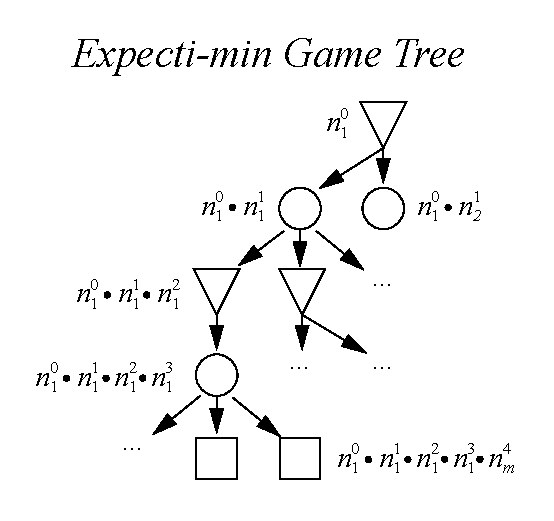
\includegraphics[width=0.49\textwidth,height=0.23\textheight,keepaspectratio]{figures/game-tree.pdf}
%  \hfill
% 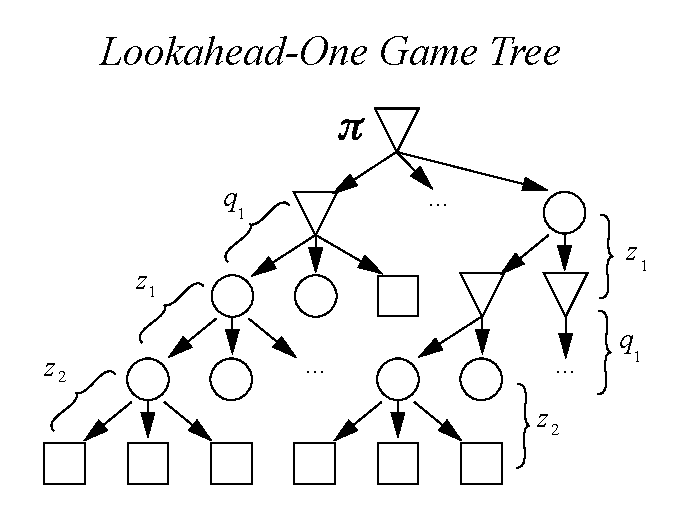
\includegraphics[width=0.49\textwidth,height=0.23\textheight,keepaspectratio]{figures/lookahead-one.pdf}
%  \caption{Monte Carlo tree search}
%\label{fig:mcts}
%\end{figure}
%
%\paragraph{Expectimin trees and optimal policies.}
%Let $\sT(\sN)$ be a expectimin tree with nodes $\sN$ (\figureref{mcts}).
%Each node $n \in \sN$ has a type $n.\sctype$ which is one of $\scmin$ (represented with inverted triangles), $\scexpect$ (represented with circles) or $\scvalue$ (represented with a square) and has children $n.\scchildren \subset \sN$.
%Additionally, nodes of type $\scvalue$ have a value $n.\scvalue$.
%The value of a node can be easily computed recursively: 
%\begin{align*}
%  \scvalue(n) &=
%  \begin{cases}
%    \min_{n'\in n.\scchildren} \scvalue(n') & \textrm{if}~n.\sctype = \scmin \\
%    \E_{n'\sim n.\scchildren}[\scvalue(n')] & \textrm{if}~n.\sctype = \scexpect \\
%    n.\scvalue & \textrm{if}~n.\sctype = \scvalue
%  \end{cases}.
%\end{align*}
%Additionally, an expectimin policy $\pi^*$ at a $\scmin$ node returns the child with the minimum value: $\pi^*(n) = \argmin_{n' \in n.\scchildren} \scvalue(n')$.
%As a concrete example, consider the expectimin tree in \figureref{mcts}. The value of the root node $n_1^0$ is,
%\begin{align*}
%  \scvalue(n_1^0) &= \min_{n_1^0.n_i^1} \E_{n_1^0.n_i^1.n_j^2} \left[\min_{n_1^0.n_i^1.n_j^2.n_k^3} \E_{n_1^0.n_i^1.n_j^2.n_k^3.n_l^4} \left[n_1^0.n_i^1.n_j^2.n_k^3.n_l^4.\scvalue \right] \right].
%\end{align*}
%
%\paragraph{Choosing queries $q_m$ with an expectimax tree.}
%Let us now formalize our decision problem as an expectimin tree, $\sT$.
%The nodes of the tree need to encapsulate as current state, the current time, $t$, the list of queries pending responses $Q = \{(q_1, t_1), \ldots, (q_m, t_m)\}$, where $q_i$ are the queries and $t_i$ is the time at which the query responds (we will compute an expectation over this quantity) and the received responses $Z = \{z_1, \ldots, z_l\}$.
%Without loss of generality, assume that $Q$ is sorted so that $t_1$ is closest in time to $t$.
%Let the root of $\sT$ be the $\min$ node $\scchoose(t, Q, Z)$, 
%with children $\scchoose(t, Q, Z).\turnin$, $\scchoose(t, Q, Z).\wait$ and $\scchoose(t, Q, Z).\query(q)$ for $q \in [n]$.
%$\scchoose(t, Q, Z).\turnin$ is a $\scvalue$ node with value equal to the expected loss of making a prediction in the current state:
%\[
%\scchoose(t, Q, Z).\turnin.\scvalue 
%= \E_{\by \sim \p(\cdot \given \bx, Z)}[\ell_{\rmclass}(\by, \byt)] + C(Q, t).
%\]
%$\scchoose(t, Q, Z).\wait$ is an $\scexpect$ node children $\{\scchoose(t', Q', Z') | t' = t_1, Q' = Q \setminus (q_1, t_1) Z' = Z \union {z_{l+1}} \forall z_{l+1} \in [L]\}$.
%Intuitively, choosing the $\wait$ node waits for the next response by advancing time and updating the query and response states.
%Finally,
%$\scchoose(t, Q, Z).\query(q)$ is an $\scexpect$ node that results in children 
%$\{\scchoose(t, Q', Z) | Q' = Q \union (q, t'), t' = t + \tau_q, \tau_q \sim \Gamma\}$: the $\query$ node places a new query and its expected time of response to $Q$. 
%
%\figureref{mcts} shows a simplified tree ignoring time constructed with a single query in flight; the root node is $\scchoose(\cdot, \{(q_1, t_1)\}, \{\})$. The branch on the left shows the expansion of the game tree along the child that chooses to query immediately, while the branch on the right considers the case where we wait to receive the first response ($z_1$) before querying ($q_2$).
%In the latter scenario, we may choose not to query again if the response we receive provides enough information.

%As described in \sectionref{model}, we would like to select and schedule several requests for labels to maximize our accuracy on predictions while trading off the cost and response time. 
%We view the problem in the Bayesian decision theoretic setting: what is the optimal behavioral policy under our current beliefs?
%The delay in the information we receive from label requests requires us to reason about time and the possible interactions between the responses we will receive.
%In this section, we describe how these interactions can be described using an expectimax tree.
%However, evaluating the optimal policy from the expectimax tree is intractable.
%We propose a Monte Carlo search based algorithm to efficiently approximate the optimal policy.

